 % !TEX root = Stanfill_CoDA.tex
\section{Data Application}\label{sec:data}

The data in our example represent the orientations of cubic crystals on a Nickel surface measured by electron backscatter diffraction. The data were obtained using a 14-fold technical replicate in each location. 
A central interest in EBSD data is the identification of so-called {\it grain maps} -- grains are defined as regions on the surface with nearly identical main direction $\bm S$. This makes the estimation of $\bm S$ crucial to the field. 


The left hand side of Figure~\ref{fig:grain-map} shows a  map of the surface colored by angle between projected median $\ProjMedian$ and the identity in each location. Distinct spatial structures become apparent.

\begin{figure}[htbp] %  figure placement: here, top, bottom, or page
   \centering
   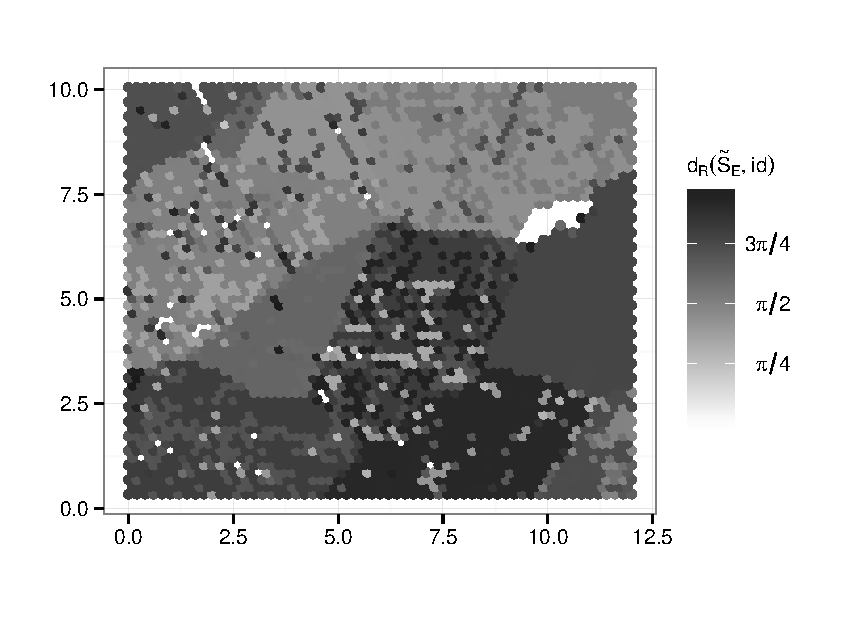
\includegraphics[width=.49\textwidth]{images/grain-map.pdf} 
   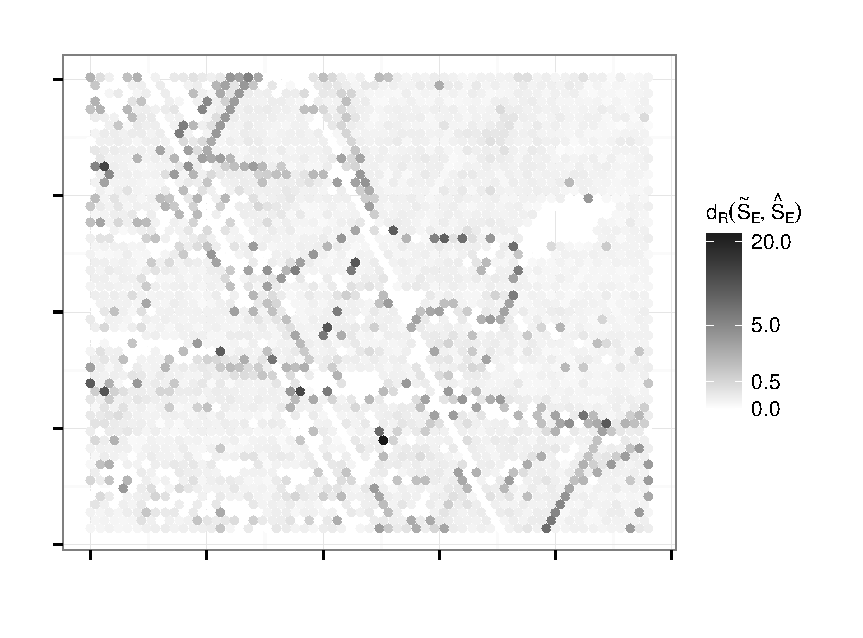
\includegraphics[width=.49\textwidth]{images/grain-diff.pdf} 
   \caption{ \label{fig:grain-map}Grain map of the investigated Nickel surface (left). Each dot corresponds to one location, shading shows the angle of the projected median estimate $\ProjMedian$ and the identity. On the right, differences between the projected median and mean estimates for each location are shown. Largest differences fall on the boundaries between grains.}
\end{figure}

% latex table generated in R 2.15.1 by xtable 1.7-0 package
% Fri Oct 26 15:44:19 2012

\begin{table}[ht]
\caption{\label{tab:rotations} List of all rotations in a single location exhibiting a large difference between mean and median estimators. We observe two tight clusters of rotations and one outlying rotation. }
\begin{center}
\scalebox{0.9}{
\begin{tabular}{rrrrrrrrrr}
  \hline
 & $x_{11}$ & $x_{12}$& $x_{13}$& $x_{21}$& $x_{22}$& $x_{23}$& $x_{31}$& $x_{32}$& $x_{33}$ \\ 
  \hline
   & -0.999 & -0.000 & -0.043 & 0.043 & 0.077 & -0.996 & 0.004 & -0.997 & 0.077 \\ 
   & -0.999 & -0.006 & -0.047 & 0.047 & 0.079 & -0.996 & 0.009 & -0.997 & 0.079 \\ 
   & -0.999 & -0.005 & -0.044 & 0.044 & 0.080 & -0.996 & 0.009 & -0.997 & 0.080 \\ 
   & -0.999 & -0.005 & -0.047 & 0.047 & 0.079 & -0.996 & 0.009 & -0.997 & 0.078 \\ 
   & -0.999 & -0.004 & -0.044 & 0.044 & 0.079 & -0.996 & 0.007 & -0.997 & 0.078 \\ 
   & -0.999 & -0.008 & -0.048 & 0.047 & 0.079 & -0.996 & 0.011 & -0.997 & 0.079 \\ 
   & -0.998 & -0.008 & -0.056 & 0.055 & 0.076 & -0.996 & 0.012 & -0.997 & 0.075 \\ 
   & -0.998 & -0.010 & -0.054 & 0.054 & 0.073 & -0.996 & 0.014 & -0.997 & 0.072 \\ [5pt]
   & -0.871 & -0.061 & -0.487 & 0.446 & 0.510 & -0.735 & 0.203 & -0.858 & 0.472 \\ 
   & -0.874 & -0.059 & -0.483 & 0.441 & 0.513 & -0.737 & 0.204 & -0.857 & 0.474 \\ 
   & -0.872 & -0.053 & -0.487 & 0.442 & 0.516 & -0.734 & 0.212 & -0.855 & 0.473 \\ 
   & -0.870 & -0.060 & -0.489 & 0.447 & 0.512 & -0.733 & 0.207 & -0.857 & 0.472 \\ 
   & -0.874 & -0.066 & -0.482 & 0.445 & 0.510 & -0.736 & 0.198 & -0.858 & 0.475 \\ [5pt] 
 & -0.708 & -0.315 & -0.632 & 0.609 & 0.181 & -0.773 & 0.358 & -0.932 & 0.063 \\ 
   \hline
\end{tabular}}
\end{center}
\end{table}
After applying all four of our estimators to each location on the surface, we noticed large differences between the estimates in some of the locations. On the right hand side of Figure \ref{fig:grain-map} the differences in angles between projected median and mean estimate for each location are shown. Largest differences are along boundaries between structures visible on the left of this figure.

Figure \ref{fig:pcp} shows a parallel coordinate plot of the data of one of these locations overlaid by the corresponding estimates: each coefficient is plotted on a vertical axis corresponding to its value in [-1,1]. Coefficients of the same matrix are connected by a line. Three clusters of rotation matrices become apparent. Note that the values are jittered -- we used a small perturbation in form of a rotation matrix with a small mis-orientation angle with respect to the identity to draw the rotation matrices in each cluster apart slightly in order to avoid over-plotting and demonstrate cluster sizes. The lines for the rotations are overlaid by the four estimates of main rotations (in color).

 Note that the figure shows a sample of a single location, yet the clustering in the data suggests clearly the presence of \emph{several} main directions. The same holds true for locations in the vicinity which happen to coincide with the boundaries between grains. 

The  median estimates, $\ProjMedian$  and $\GeomMedian$, are not nearly as much affected by the clustering in the sample as are the means, and reliably estimate the main direction of the largest group of rotations within the sample.

%\begin{figure}[htbp] %  figure placement: here, top, bottom, or page
%   \centering
%   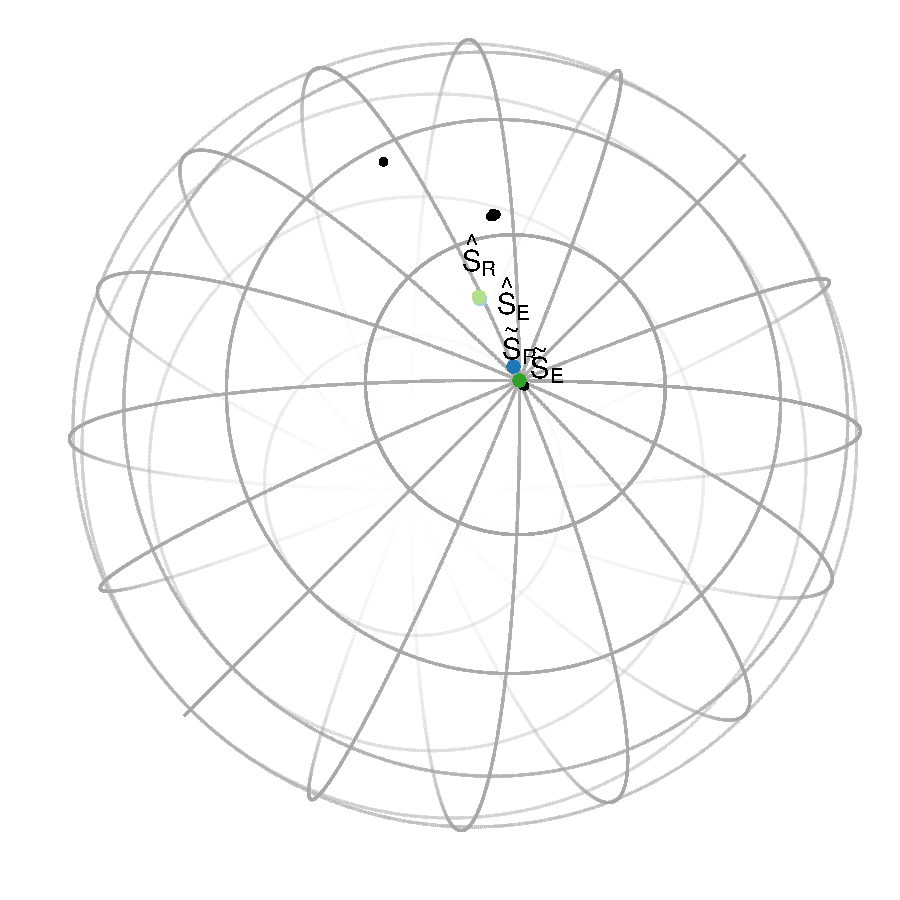
\includegraphics[width=.275\textwidth]{images/eyeball-1031-1.pdf} 
%   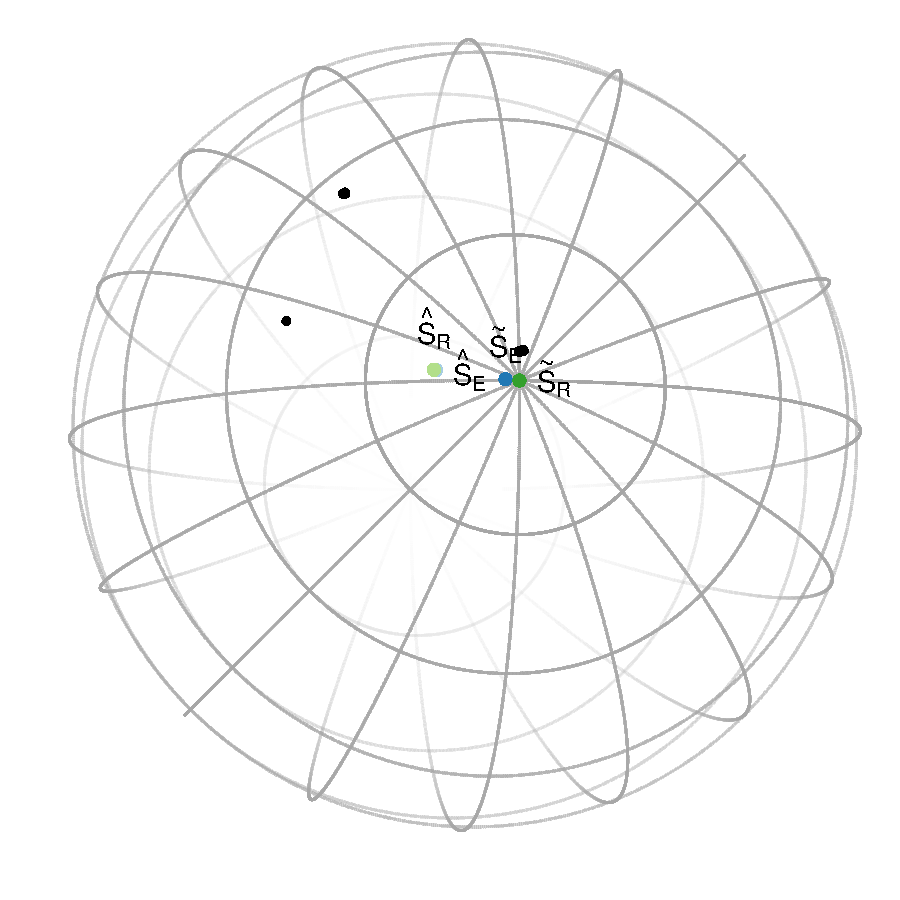
\includegraphics[width=.275\textwidth]{images/eyeball-1031-2.pdf} 
%   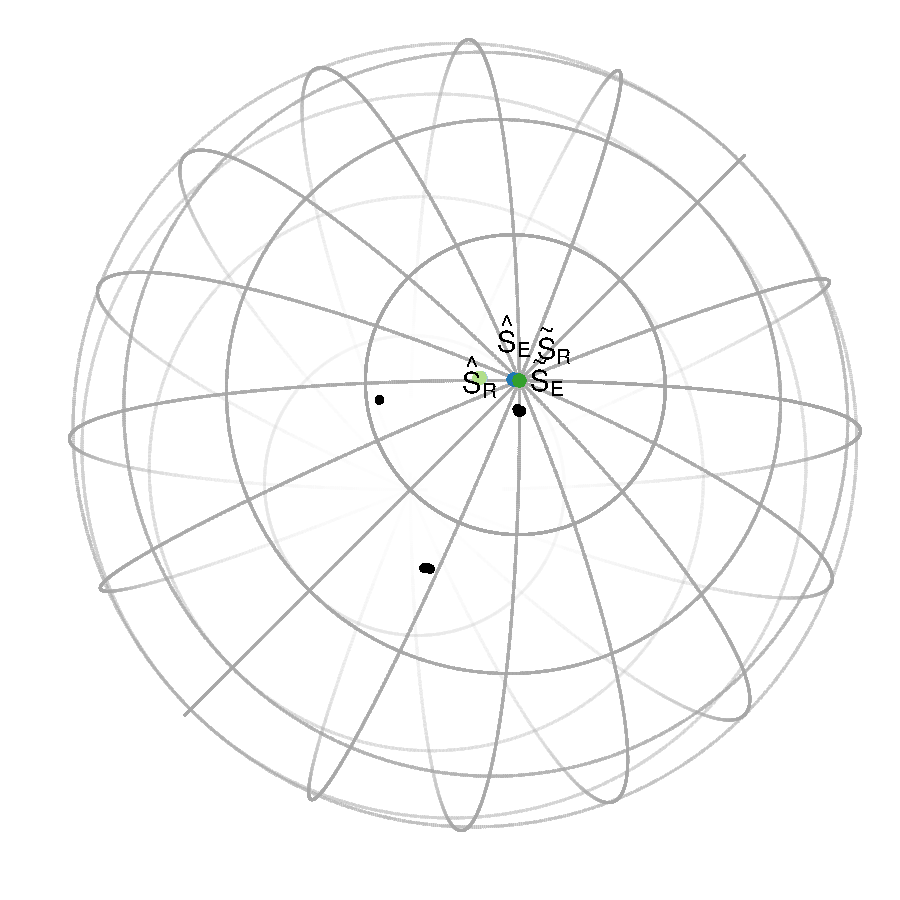
\includegraphics[width=.275\textwidth]{images/eyeball-1031-3.pdf} 
%   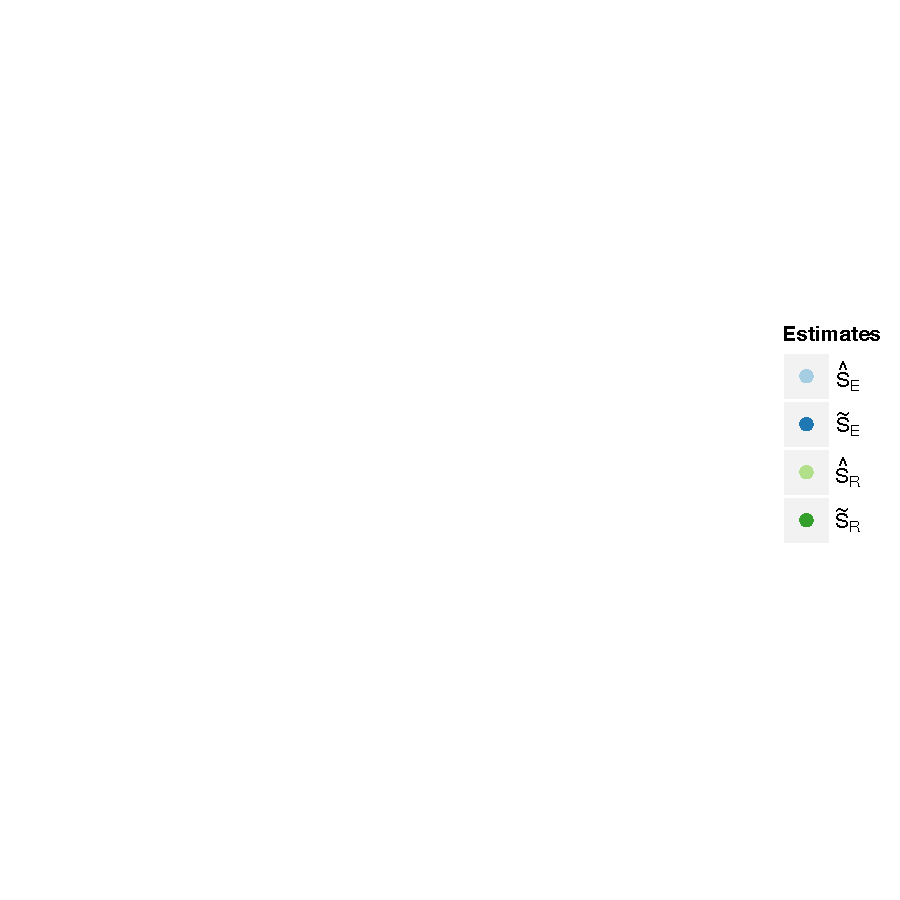
\includegraphics[height=.275\textwidth]{images/legend.pdf} 
%   \caption{ \label{fig:eyeballs-1}Sphere plots of EBSD measurements at a single location. The data sample is shown as dark grey points, the estimates of the main direction are colored and labelled. The clustering of the results makes the existence  of several main directions  quite obvious. }
%\end{figure}

\begin{figure}[htbp] %  figure placement: here, top, bottom, or page
   \centering
   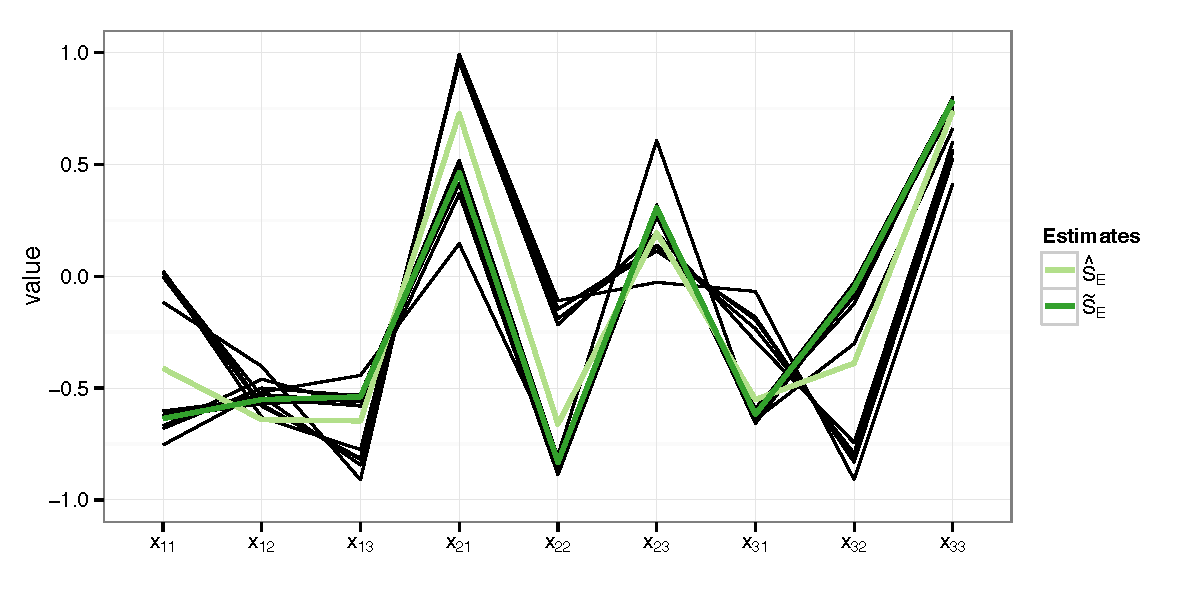
\includegraphics[width=.7\textwidth]{images/pcp.pdf} 
   \caption{ \label{fig:pcp}Parallel coordinate plot of all nine coefficients of the rotation matrices in a single location. Three clusters of rotation matrices are apparent.  }
\end{figure}



